\documentclass[a4paper,11pt]{jlreq}
% 基本とドライバ関連
\usepackage{graphicx}
\usepackage{xcolor}
\usepackage{makeidx}
\usepackage{ascmac}

% LuaTeX-ja設定
\usepackage{luatexja}% 日本語したい
\usepackage[haranoaji,no-math,deluxe,expert,nfssonly,match,scale=1.0]{luatexja-preset}
\renewcommand{\kanjifamilydefault}{\gtdefault}% 既定をゴシック体に
\usepackage{lltjext}

% 数式系基本
\usepackage{amsmath}
\usepackage{amsthm}
\usepackage{amssymb}
\usepackage{mathtools}
% \mathtoolsset{showonlyrefs=true}
\usepackage{derivative}
\usepackage[b]{esvect}
\usepackage{nicematrix}
\usepackage{siunitx}
\usepackage{bm}

% 画像関係
\usepackage{animate}
\usepackage{svg}
\usepackage{tikz}

%表関連
\usepackage{multirow}

% 自然科学用追加
% \usepackage{chemmacros}
% \usechemmodule{all}
% \selectchemgreekmapping{fontspec}
\usepackage{chemfig}
\setchemfig{atom sep=1.5em}
% \ifdraft{}{\setchemfig{bond join=true}}

% 数式フォント設定
\usepackage{anyfontsize}
\newcommand{\sfscale}{0.98}
\newcommand{\ttscale}{0.96}
% \usepackage[mathnoalias]{iwona}
% % \setmainfont{Iwona}
% \usepackage[scale=\sfscale]{roboto}
% \usepackage[scale=\ttscale]{roboto-mono}
% \usepackage{BOONDOX-uprscr}
% \usepackage{BOONDOX-ds}

% ページ設定
\usepackage{geometry}
\geometry{left=25truemm, right=25truemm, top=25truemm, bottom=25truemm}
% \pagestyle{empty}

% hyperref関連
\usepackage{bookmark}
\usepackage{xurl}
\hypersetup{unicode,bookmarksnumbered=true,colorlinks=true,final}

%%%%%%%%%%%%%%%%%%%%%%%
\graphicspath{{../figure/}{../../figure/}}

\usepackage{xr}
\externaldocument{./polymer_models_exam}

\begin{document}
\section{粗視化モデルでの高分子の大きさ}
\label{sec:CG_model}

前章で、高分子鎖の振る舞いについてミクロな化学的視点からスタートして考察し、非常に細長い紐が丸まっているというイメージを持つことができた。
このイメージを、材料としての特性と関連付けていくためには、この「丸まった紐のかたまり」を、何らかの形で定義する必要がある。

前章において、各ボンドがトランス配座を取り直線状に伸びた場合の伸び切り構造の長さという1つの特徴長さについての議論は既に行った。
ここでは、丸まった紐を記述するために、丸まった状態での長さを決めていく方法について確認しよう。
長さが決まれば、そのかたまりの占める空間の体積はその長さの三乗程度で見積もることができるようになる。

最初に、両末端の距離について考察しよう。
セグメントが目に見えるようなモデルで考えるには、このような長さは便利であるが、実際にはこの長さを実測することは困難です。
続いて、実測が容易である慣性半径という重心からの距離に対応するような長さについて考察して、末端間距離との関係を確認する。
なお、前章で示したようなミクロな構造を考慮していたのでは、自由度が大きすぎて議論が困難であるので、大胆に粗視化した自由連結鎖というモデルを用いてスタートすることになる。

モデルの妥当性とついての議論を行った後、最後に、高分子物理で取り扱いが容易であるガウス鎖というモデルについて簡単に説明する。

%\subsection{空間的な大きさの各種モデル}
%

%しかしながら、前述のように、単純な回転異性体モデルでも、その取りうる場合の数は分子量の増加に伴い指数関数的に増加するので、その厳密な取り扱いは非常に困難になる。
%したがって、さらに簡易化した統計的なモデルとして取り扱う必要がある。

\subsection{高分子鎖の大きさ}

ここでは、実在の高分子のモノマー連鎖のことは一旦忘れて、セグメントという球が、長さ $a$ のボンドで連結しているという仮想的なモデルを考えよう。
なお、セグメントは、自由に折れ曲がることのできる単なる結節点として取り扱い、その体積は考えないこととする
\footnote
{
このモデル化の妥当性についても、きちんと議論できるのであるが、ここでは天下りにこういうモデルでの記述できるということにしていただきたい。
}。
このようなモデルは、「自由連結鎖」、あるいは、「ランダム・フライト・モデル」と呼ばれる。

さらに、簡単のために、直鎖上のポリマーを対象として、$N+1$ 個のセグメント(一方の端から、0, 1, $\cdots$, N と番号を付ける)が、$N$ 本のボンドにより一本の紐のように連結していることとする。

以下に、1000 個のセグメントからなる自由連結鎖を二次元平面上に記述した例を示した
\footnote
{
この図は、一方の端のセグメントから単位長さのボンドをランダムに発生させ、次々とつなげて作成したものである。
自由連結鎖のように一定長さのボンドベクトルを任意の方向に発生させるためには、三角関数をうまく使えばよい。(章末問題 \ref{it:3-1})
}。
\begin{figure}[htb]
	\begin{center}
		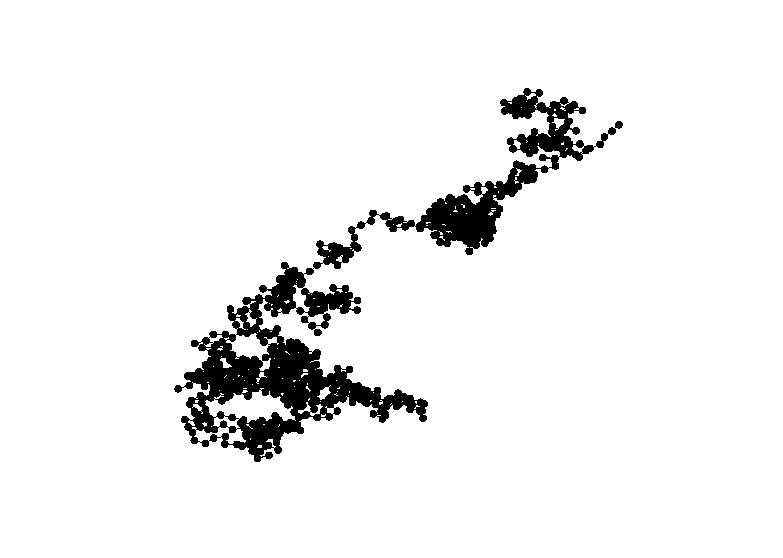
\includegraphics[width=10cm]{RF.eps}
		\caption{自由連結鎖の例(1000 セグメント)}
		\label{fig: RF}
	\end{center}
\end{figure}

自由連結鎖モデルを用いて、「末端間距離」および「慣性半径」という二つの長さについて考えてみよう。

\subsubsection{末端間距離 $R$}

これは、鎖の両末端のセグメント(0 番目と $N$ 番目)との間にベクトル $\bm{R}$ を考え、その二乗の平均 $\langle |\bm{R}|^2 \rangle$ (平均二乗末端間距離)を用いて、下式で定義されるものである(章末問題 \ref{it:3-2})。
\begin{equation}
R=\sqrt{\langle |\bm{R}|^2 \rangle}
\end{equation}

前述の自由連結鎖の例における末端間ベクトルを以下に図示した。
\begin{figure}[htb]
	\begin{center}
		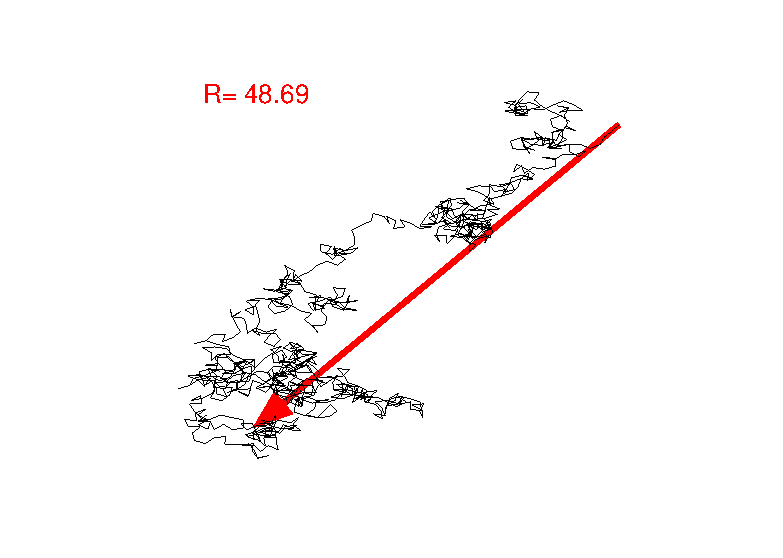
\includegraphics[width=10cm]{RF_EV.eps}
		\caption{末端間ベクトルの例}
		\label{fig: RF_EV}
	\end{center}
\end{figure}

このモデルにおいて、ボンドが自由に連結しているという性質を用いることにより、末端間距離は、以下のように求めることができる。
\begin{align}
R^2
	&= \langle |\bm{R}|^2 \rangle \notag \\
	&=\langle |\bm{r}_0 - \bm{r}_N|^2 \rangle \notag \\
	&=\langle |(\bm{r}_1 - \bm{r}_0) + (\bm{r}_2 - \bm{r}_1) + \cdots + (\bm{r}_N - \bm{r}_{N-1})|^2 \rangle \notag \\
	&=\langle |\bm{u}_0 + \bm{u}_1 + \cdots + \bm{u}_{N-1}|^2 \rangle \notag \\
	&=\left\langle \left|\sum_{i=0}^{N-1}\bm{u}_i \right|^2 \right\rangle \notag \\
	&= 
		[ 
		{\color{red} |\bm{u}_0|^2} + \langle \bm{u}_0 \cdot \bm{u}_1 \rangle + \langle \bm{u}_0 \cdot \bm{u}_2 \rangle + \cdots + \langle \bm{u}_0 \cdot \bm{u}_{N-1} \rangle 
		] \notag \\
	&\quad+ 
		[ 
		\langle \bm{u}_1 \cdot \bm{u}_0 \rangle + {\color{red} |\bm{u}_1|^2} + \langle \bm{u}_1 \cdot \bm{u}_2 \rangle + \cdots + \langle \bm{u}_1 \cdot \bm{u}_{N-1} \rangle 
		] \notag \\
	&\quad\quad \vdots \notag \\
	&\quad+ 
		[ 
		\langle \bm{u}_{N-1} \cdot \bm{u}_0 \rangle + \langle \bm{u}_{N-1} \cdot \bm{u}_1 \rangle + \cdots + \langle \bm{u}_{N-1} \cdot \bm{u}_{N-2} \rangle + {\color{red} |\bm{u}_{N-1}|^2} 
		] \notag \\
	&=\sum_{i=0}^{N-1} \left\langle \left|\bm{u}_i \right|^2 \right\rangle 
	+\sum_{i \neq j} \left\langle \bm{u}_i \cdot \bm{u}_j \right\rangle \notag \\
	&= N a^2 \notag \\
\therefore R &= N^{1/2}a
\label{eq:r2}
\end{align}
なお、$\bm{r}_i$ は $i$ 番目のセグメントの位置ベクトルを表しており、$\bm{u}_i \equiv \bm{r}_{i+1} - \bm{r}_i$ はボンドベクトルを表している(章末問題 \ref{it:3-3})。

\subsubsection{慣性半径 $R_g$}

慣性半径 $R_g$ は、鎖の重心 $\bm{r}_g$ から各セグメントまでの距離の二乗平均の平方根として以下のように定義される
\footnote
{
任意の基準点から見た $i$ 番目のセグメントの位置ベクトルを $\bm{r}_i$ で指定した場合、この高分子鎖の重心 $\bm{r}_g$ は、以下のように定義することができる。
\begin{equation*}
\bm{r}_g = \dfrac{1}{N+1} \sum_{j=0}^{N} \bm{r}_j
\end{equation*}

なお、この定義は、セグメントの重量を単位量 1 と見た場合の、剛体の力学における慣性モーメントと同等であると考えれば理解しやすい。
}。
\begin{equation*}
R_g^2 = \dfrac{1}{N+1} \left\langle \sum_{i=0}^{N} |\bm{r}_i - \bm{r}_g|^2 \right\rangle
\end{equation*}

直鎖高分子では、慣性半径は以下のように記述されることになる
\footnote
{
この導出については、\ref{sec:rg}に詳細を記したので、そちらを見ていただきたい。
}。
\begin{align}
R_g^2 = \dfrac{1}{6}Na^2 = \dfrac{1}{6} R^2
\label{eq:rg_r}
\end{align}

以下に、前述の自由連結鎖モデルにおいて、慣性半径で円を描いた図を示した。
なお、中心の大きい赤丸が重心を表している。

慣性半径が、高分子鎖の空間的な広がりの半径にほぼ相当し、高分子鎖の大体の大きさを表していることがイメージできる。
\begin{figure}[htb]
 \centering
	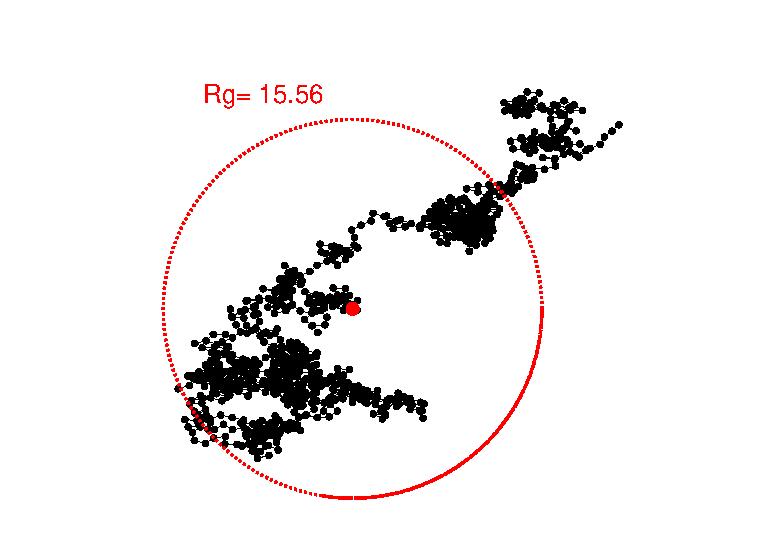
\includegraphics[width=10cm]{RF_Rg.eps}
	\caption{自由連結鎖の慣性半径}
	\label{fig: RF_Rg}
\end{figure}

実際の測定においては、高分子鎖の末端を見出すことは困難で特定の条件がそろわない限り
\footnote
{
高分子鎖の一端から逆の端まで双極子モーメントの向きがそろったようなポリマーを対象とした誘電測定により末端間距離を測定できる場合があるが、こういう系は特殊である。
}、末端間距離 $R$ を実測することは困難である。
一方、慣性半径 $R_g$ は光散乱測定により実測することが可能である。
したがって、必要に応じて、慣性半径 $R_g$ を測定して (\ref{eq:rg_r}) 式の関係を通して末端間距離 $R$ へと換算することが可能である。

\subsection{高分子鎖のモデル}

ここでは、仮想的なセグメントを用いて記述された自由連結鎖という抽象的なモデルと、実際の分子に近いモデルとの関連について、もう少しだけ考察しよう。

前述の自由連結鎖においては、ボンドの角度についての規制を全く考慮していなかった。
しかしながら、実際のポリマー鎖においては、二つの\chemfig{C-C}結合の間には結合角が存在する。
さらには、結合が連結していることにより、以前にニューマン投影式を用いて議論したようにその結合周りの回転も束縛を受けていることになる。

このような拘束条件を考慮したモデルとして、C-C 結合の結合角だけを考慮した「自由回転鎖」モデル、および、配座に応じた回転の束縛を考慮した「束縛回転鎖」モデルの二つがよく知られている。

自由回転鎖モデルでの平均二乗末端間距離 $R_{fr}^2$ は、以下のように表記される
\footnote
{
この導出については、\ref{sec:1FR_R2} を参照されたい。
}。
\begin{align}
R_{fr}^2 = Na^2 \dfrac{1+\cos \theta}{1-\cos \theta}
\label{eq:r2_sokubaku}
\end{align}

具体的な $\theta$ の値として、前述の $\theta = 180-109.5= 70.5^o$ を用いる
\footnote
{
ボンドベクトルの成す角であるので、C-C 結合の結合角 $109.5^o$ の外角となることに注意。
}と、$R_{fr}^2 \simeq 2 \times R^2$ となり、自由連結鎖の末端間距離の $\sqrt{2}$ 倍に増加することが判る。


一方、束縛回転鎖モデルでは、以下のように表すことができる(導出および詳細な議論は省略する)。
\begin{align}
R_{rr}^2 = Na^2 \dfrac{1+\cos \theta}{1-\cos \theta} \dfrac{1+ \langle \cos \theta \rangle}{1- \langle \cos \theta \rangle}
\label{eq:r2_sokubaku}
\end{align}
ここで、
\begin{align}
\langle \cos \theta \rangle = \dfrac{\displaystyle \int_0^{2 \pi} \cos \phi \exp [-u(\phi)/k_B T] d \phi}{\displaystyle \int_0^{2\pi} \exp [-u(\phi)/k_B T] d \phi}
\end{align}

(\ref{eq:r2_sokubaku}) 式に表れた $Na^2$ にかかる係数項($\cos \theta$ および $\langle \cos \theta \rangle$ に関する分数の因子)は、「束縛回転鎖」モデルにおいても、定数項として取り扱えるので、結局、
自由回転鎖モデルと同様に、末端間距離の増加という因子として働くことになる。

したがって、現実のポリマー鎖に近くなるように結合角を考慮した場合でも、末端間距離は、$N^{1/2}$ に比例する(比例定数は $> 1$ となっている)ことが確認できる。
なお、この比例定数に対応するものが、特性比 $C_{\infty}$ であり、このことについては後ほど議論する。

\subsection{ガウス鎖について}

ここまでに示したように、高分子の主鎖を形成するボンドは熱運動のために、非常に多くの配座(コンフォメーション)を取ることができるのであった(極低温は除く)。
このような状態を考慮した場合、末端間距離の平均は分子量の $1/2$ 乗に比例し、かつ、その分布 $P(\bm{R})$ は、ガウス分布
\footnote
{
ガウス分布については、\ref{sec:gauss} を参照していただきたい。
}に従うことを示すことができる(導出は省略)。
\begin{align}
P(\bm{R}) =\left( \dfrac{3}{2 \pi N b_0^2} \right)^{3/2} \exp \left[ -\dfrac{3|\bm{R}|^2}{2Nb_0^2} \right]
\end{align}

高分子鎖が十分に長いと考えた場合、その一部分だけを取り出した部分鎖の末端間距離もガウス分布に従うと考えることができるようになる。
このように、部分鎖と全体とを比べても、スケールフリーに同様なガウス性を有するポリマー鎖をガウス鎖と呼んでいる。

\end{document}